\documentclass[letterpaper,11pt]{article}
\usepackage[letterpaper,margin=1in]{geometry}



\usepackage{amsmath,amssymb,amstext,amsthm} % Lots of math symbols and environments
\usepackage[pdftex]{graphicx} % For including graphics N.B. pdftex graphics driver 
\usepackage{picins}
\usepackage[pdftex,letterpaper=true,pagebackref=false]{hyperref} 

\hypersetup{	% override some previously defined hyperref options
%    colorlinks,%
    citecolor=black,%
    filecolor=black,%
    linkcolor=black,%
    urlcolor=black}

\usepackage{bbm}
\usepackage{mathbbol}
\usepackage[algosection,ruled,lined,linesnumbered,longend]{algorithm2e}
\usepackage{algorithmic}
\usepackage{latexsym}
\usepackage{wrapfig}
\usepackage{float}
\usepackage{caption}
\usepackage{subcaption}

\newcommand{\cmd}[1]{\ensuremath{\mbox{\bf #1}}} 
\newcommand{\vio}{\ensuremath{\cmd{violation}}}
\newcommand{\st}{\ensuremath{\mbox{s.t.}}}
\newcommand{\red}[1]{\textcolor{red}{#1}}
\newcommand{\beq}{\begin{equation}}
\newcommand{\bet}{\begin{table}}
\newcommand{\eeq}{\end{equation}}
\newcommand{\real}{\mathbb{R}} %IMPORTANT
\newtheorem{theorem}{Theorem}[section]
\newtheorem{lemma}[theorem]{Lemma}
\newtheorem{definition}[theorem]{Definition}
\newtheorem{corollary}[theorem]{Corollary}
\newtheorem{example}[theorem]{Example}
\newtheorem{nmbrs}[theorem]{Numbering}
\newtheorem{assump}[theorem]{Assumption}
\newtheorem{prop}[theorem]{Proposition}
\newtheorem{prob}[theorem]{Problem}
\newtheorem{lem}[theorem]{Lemma}
\newtheorem{thm}[theorem]{Theorem}
\newtheorem{cor}[theorem]{Corollary}
\newtheorem{rem}[theorem]{Remark}
\newtheorem{remark}[theorem]{Remark}
\newtheorem{conj}[theorem]{Conjecture}
\newtheorem{alg}[theorem]{Algorithm}
\newtheorem{ex}[theorem]{Exercise}
\newtheorem{problem}[theorem]{Problem}
\newtheorem{result}[theorem]{Result}
\newtheorem{claim}[theorem]{Claim}
\newtheorem{coroll}[theorem]{Corollary}
\newtheorem{theo}[theorem]{Theorem}
\newtheorem{defin}[theorem]{Definition}
\newtheorem{nota}[theorem]{Notation}

\def\cA{{\mathcal{A}}}
\def\cS{{\mathcal{S}}}
\def\R{\mathbb{R}}
\def\M{\mathbb{M}}
\def\C{\mathbb{C}}
\def\Z{\mathbb{Z}}
\def\Rnbyn{\R^{n\times n}}
\def\Rn{\mathbb{R}^n}
\def\Rm{\mathbb{R}^m}
\def\Ss{\mathcal{S}}

\DeclareMathOperator{\kvec}{{vec}}
\DeclareMathOperator{\adj}{{adj}}
\DeclareMathOperator{\trace}{{trace}}
\DeclareMathOperator{\argmin}{{argmin}}
\DeclareMathOperator{\argmax}{{argmax}}
\DeclareMathOperator{\arrow}{{arrow}}
\DeclareMathOperator{\ext}{{ext}}
\DeclareMathOperator{\reshape}{{reshape}}
%\DeclareMathOperator{\deg}{{deg}}
\DeclareMathOperator{\cut}{{cut}}
\DeclareMathOperator{\blkdiag}{{blkdiag}}
\DeclareMathOperator{\tr}{{tr}}
\DeclareMathOperator{\Diag}{{Diag}}
\DeclareMathOperator{\diag}{{diag}}
\DeclareMathOperator{\dDiag}{{dDiag}}
\DeclareMathOperator{\Ddiag}{{Ddiag}}
\DeclareMathOperator{\Mat}{{Mat}}
\DeclareMathOperator{\offDiag}{{offDiag}}
\DeclareMathOperator{\usMat}{{us2Mat}}
\DeclareMathOperator{\usvec}{{us2vec}}
\DeclareMathOperator{\svec}{{s2vec}}
\DeclareMathOperator{\vsvec}{{vs2vec}}
\DeclareMathOperator{\dsvec}{{dsvec}}
\DeclareMathOperator{\Hmat}{{Hmat}}
\DeclareMathOperator{\vSmat}{{vSmat}}
\DeclareMathOperator{\Smat}{{S2mat}}
\DeclareMathOperator{\sMat}{{s2Mat}}
\DeclareMathOperator{\hMat}{{hMat}}
\DeclareMathOperator{\vsMat}{{vs2Mat}}
\DeclareMathOperator{\kmat}{{Mat}}
\DeclareMathOperator{\sdiag}{{sdiag}}
\DeclareMathOperator{\Kprod}{\otimes}
\DeclareMathOperator{\Kcal}{{\mathcal K}}
\DeclareMathOperator{\Hcal}{{\mathcal H}}
\DeclareMathOperator{\relint}{{relint}}
\DeclareMathOperator{\nullity}{{null}}
\DeclareMathOperator{\rank}{{rank}}
\DeclareMathOperator{\cond}{{cond}}
\DeclareMathOperator{\conv}{{conv}}
\DeclareMathOperator{\AUT}{{AUT}}
%\DeclareMathOperator{\par}{{part}} 

\newcommand{\Sn}[1][]{\mathcal{S}^{\ifthenelse{\equal{#1}{}}{n}{#1}}}
\newcommand{\Sk}[1][]{\mathcal{S}^{\ifthenelse{\equal{#1}{}}{k}{#1}}}
\newcommand{\Snp}[1][]{\mathcal{S}_+^{\ifthenelse{\equal{#1}{}}{n}{#1}}}
\newcommand{\Skp}[1][]{\mathcal{S}_+^{\ifthenelse{\equal{#1}{}}{k}{#1}}}
\newcommand{\Snpp}[1][]{\mathcal{S}_{++}^{\ifthenelse{\equal{#1}{}}{n}{#1}}}
\newcommand{\MM}{{\mathcal M}}
\newcommand{\QQ}{{\mathcal Q}}
\newcommand{\NN}{{\mathcal N} }
\newcommand{\EE}{{\mathcal E} }
\newcommand{\LL}{{\mathcal L} }
\newcommand{\KK}{{\mathcal K} }
\newcommand{\RR}{{\mathcal R} }
\newcommand{\FF}{{\mathcal F} }
\newcommand{\Fk}{{\mathcal F}_k}
\newcommand{\DD}{{\mathcal D} }
\newcommand{\BB}{{\mathcal B} }
\newcommand{\CC}{{\ensuremath{\mathcal C}}}
\newcommand{\GG}{{\mathcal G} }
\newcommand{\OO}{{\mathcal O} }
\newcommand{\PP}{{\mathcal P} }
\newcommand{\TT}{{\mathcal T} }
\newcommand{\UU}{{\mathcal U} }
\newcommand{\HH}{{\mathcal H} }
\newcommand{\VV}{{\mathcal V} }
\newcommand{\ZZ}{{\mathcal Z} }
\newcommand{\WW}{{\mathcal W} }
\newcommand{\SDP}{{\bf{\rm SDP\,}}}
\newcommand{\SDPs}{{\bf{\rm SDPs\,}}}
\newcommand{\SDPns}{{\bf{\rm SDP}}}
\newcommand{\LP}{{\bf{\rm LP\,}}}
\newcommand{\Mm}{{\mathcal{M}_m}}
\newcommand{\0}{\mathbb{0}}
\newcommand{\1}{\mathbb{1}}

\newcommand{\textdef}[1]{\textit{#1}\index{#1}}

\title{A 7 Approximation for Hitting the Even Cycles of a Planar Graph}

\begin{document}
\begin{Large}
\begin{center}
    A 7 Approximation for Hitting the Even Cycles of a Planar Graph
\end{center}
\end{Large}

\section{Introduction}
In this short note we present a constant-factor approximation algorithm for the {\em even-cycle transversal} (ECT) problem:
Given a planar graph $G=(V,E)$ and weights $w:V \rightarrow \mathbb{R}_+$ find a minimum weight set $H \subset V$ such that $C \cap H \neq \emptyset$ for all even cycles $C$ in $G$.   
The problem of hitting all cycles has a 2 approximation \cite{Becker2apx}   and a PTAS \cite{Fomin2010} .   \cite{GW98}  consider for planar graphs, a  more general problem where we are given a set of  cycles $\mathcal{C} $ satisfying some ``uncrossing property" (see \cite{GW98} ) is given and we wish to find a minimum weight set $H \subset V$ of vertices, such that  $C \cap H \neq \emptyset $   for all $C \in \mathcal{C}$.  They give a 3 approximation algorithm for this problem in planar graphs and propose an improved approximation using a so called ``pocket oracle" which they claim is a 9/4 approximation.   \cite{BY12}   show that the approximation of the pocket oracle proposed in \cite{GW98} is not 9/4, but 18/7 instead and also give a 2.4  approximation algorithm using a new ``three-pocket oracle".
The approach presented here uses the primal-dual framework of Goemans and Williamson~\cite{GW97,GW98}.

\section{Even cycles}

In the following, we fix an embedding of graph $G$. For a cycle $M$ in $G$, we let $f(M)$ be the faces in the interior region of $M$. Given a family \CC\ of cycles, a cycle $M \in \CC$ is {\em face-minimal} (with respect to \CC) if there is no $M' \in \CC$ with $f(M') \subsetneq f(M)$.
In the following, we also abuse notation slightly,
and use $A \subset B$ as a short-hand for graph $A$ being a subgraph of graph $B$. The following lemma captures a key property for our algorithm.

\begin{lemma}
Let C be a face minimal even cycle of our graph, then $C$ contains at most 2 faces of our graph.  
\end{lemma}
\begin{proof}
Let $F_1, F_2 ,,.. F_l$ be the faces of C assume for a contradiction $l \geq 3$ then $ |E(C)| = |E(F_1)|+|E(F_2)|+..+|E(F_l)| \ \ \ \ \text{mod \ \ 2} $.  Thus if $l$ is odd one of the faces of $C$ must be even. If $l \geq 4$ is even, then remove a path $P \subset E $ bordering 2 faces of $C$ in $G \backslash P$ , \ \ $C$ has $l-1$ faces $ F_1', F_2' ,... , F_{l-1}' $ , \ \ \ $l-1 \geq 3 $ is odd and one of the $F_i'$ is even. This cycle is strictly contained in $C$ contradiction.
\end{proof} 

The above lemma easily implies that the set of face-minimal even cycles can be found efficiently by 
checking all even faces, and all adjoining faces in $G$. Suppose that our goal is to hit a set $\mathcal{C}$ of cycles. The algorithm presented here is then based on the following natural pair of linear programs.

\medskip
\noindent\hspace*{-4ex}
\begin{minipage}{.47\textwidth}
\begin{align}
    \min ~~ & \sum_{v \in V} w_x x_v \tag{P} \label{primal}\\
    \st ~~ & \sum_{v \in C} x_v \geq 1 ~~ \forall C \in \mathcal{C} \notag\\
    & x \geq \0 \notag
\end{align}
\end{minipage}
\hspace*{.02\textwidth}
\vrule
\hspace*{.02\textwidth}
\begin{minipage}{.47\textwidth}
\begin{align}
\max ~~ & \sum_{C \in \mathcal{C} } y_C \tag{D} \label{dual} \\
\st ~~ &  \sum_{C:  \ v \in C} y_C \leq w_v ~~ \forall v \in V\notag \\
& y \geq \0 \notag
\end{align}
\end{minipage}
\medskip

In the following we state the classical primal-dual framework for feedback vertex set problems as was previously described by Goemans and Williamson~\cite{GW97,GW98}. In the algorithm, we use $u \bullet M$ as a short for "{\em $u$ is a vertex on cycle $M$}", and we use $\vio(G,\CC,S)$ to denote a call to a so called {\em violation oracle} that, given a graph $G$, cycles \CC, and a partial solution $S$, returns a {\em minimal} collection of cycles that are not hit by $S$.

\medskip

\begin{algorithm}[H]
\caption{\cite{GW98}\label{pdalg} Generic primal-dual algorithm 
    for feedback vertex set problem given by $(G(V, E), w, \mathcal{C} )  $  }
\begin{algorithmic}
 \STATE $y  =  0$   
 \STATE Let $w(y,u) =  w(u) -  \sum_{{M \in \mathcal{M} : u \bullet M}}   y_M $ 
 \STATE $S = \{u \in V :   w(u) = 0 \}$
\WHILE{$S$ is not a hitting set for $\mathcal{C}$} 
\STATE  $\MM= \vio(G, \CC, S)$.
\STATE $c_{ \MM (u) } \leftarrow |{M \in \MM : u \bullet M}|, \forall u \in V $.
 \STATE $ \alpha 
\leftarrow \text{min}_ {u \in V \backslash S} | w(y,u)| /
c_{\MM(u) } $ 
\STATE  $y_M = y_M + \alpha$, for all $M \in \MM$
$ S \leftarrow \{u \in V :  w(y,u) = 0 \}. $
\ENDWHILE 
\RETURN a minimal hitting set $ H \subset S $ of $\mathcal{C}$.
\end{algorithmic}
\end{algorithm} 

\medskip

In \cite{GW98}, the set $\mathcal{C}$ is the set of all directed cycles in a directed planar graph. For us, $\mathcal{C}$ is the set of even cycles in an undirected planar graph $G$. Given a partial hitting set $S \subseteq V$, our oracle \vio\ will return a maximal set of face-minimal even cycles. 
\begin{lemma}[\cite{GW98}]\label{approx} 
Suppose that Algorithm \ref{pdalg} returns solution $F \subseteq V$, and that it generates minimally violated sets of cycles $\MM_1, \ldots, \MM_q$ during its execution.
$F$ is an $\alpha$-approximate solution if 
\[ \sum_{M \in \MM_i} |F \cap M| \leq \alpha|\MM_i|,
 \] 
for all $1 \leq i \leq q$.
\end{lemma}

Consider an inclusion-wise minimal hitting set $H \subseteq V$. Then note that the minimality of $H$ implies that, for each $h \in H$, there is at least one $M_h \in \CC$ such that $h$ is the only $H$-vertex on $M_h$. We call such a cycle $M_h$ a {\em witness cycle} of $h$. 

\begin{definition}
For a hitting set $H \subset V$, $ \mathcal{M} $ a set of face-minimal cycles of our graph, define  the debit graph $B= ( \mathcal{M} \cup H, E  ) $. Where $ (M,h) \in E $ if node $h$ is on cycle $M$.  
\end{definition} 
Like in \cite{GW98},  we will sometimes think of our debit graph as drawn (embedded in the plane) with the node $v_M$ for cycle $M$ (in debit graph) located at the center of the cycle $M$ (in G) (nodes $h$ where they are in the original graph $G$).       In \cite{GW98}   for the case of all faces the debit graph is planar we will show this also happens to be the case here.
Notice that $\sum_{C \in \mathcal{M} } |H \cap C| = |E(B) |.
 $  % then for each $ h \in H $ let  $M_h  \in M $ be a witness cycle for the node $h$  and let $A$ be the set of witness cycles,  consider $B' = B[ M \backslash A ] $  % \ \ \  $ |V(B')| = |V(B) | - |A|  $  \ \ \ $|E(B')| = |E(B) | - |A|  $  

The following is an easy 3 approximation for GW in planar graphs if each witness cycle was incremented in our iteration.

\begin{lemma}\label{debit}
For a bipartite planar graph $G= (A ,B) $ such that for each node $b  \in B $ is incident to a node of degree 1 in A then $|E(G) | \leq  3|A| $.
\end{lemma}
\begin{proof}
Let for each $b \in B$ choose a node $a_b \in A$  of degree 1 and denote $ A' := \{ a_b  \ \ \ b \in B  \} $ and consider $ G' = G[ (A \backslash A' \cup B) $ applying Euler's formula (for bipartite planar graphs) to G' we get $E(G') \leq 2 |A \backslash A' \cup B|$. Since  $E(G) = E(G')+ | A'| \leq  |A'|+ 2 |A \backslash A' \cup B|  \leq 2|A|+ |A'| \leq 3|A|$.
\end{proof}  

\begin{corollary}\label{lack witness}
In Lemma \ref{debit} if at most k nodes of B  in \ \ G=(A,B) are not incident to nodes of degree 1 then $|E(G) | \leq  (3 + 3k/|A| )|A| $.
\end{corollary}
\begin{proof}
Construct G' from B by adding k nodes of deg 1  to the A side of G.  $ |E(G')| \leq 3(| A |+k )  \leq (3 + 3k/|A| ) |A| $
\end{proof}

Note that this gives an easy 3 apx for instances of planar FVS where all witness cycles of our hitting set, for each iteration is a cycle incremented in our iteration.   In the following arguments  we will think of  paths and cycles as being subgraphs and for graph $H$ and path $P$  use the convention $ H \backslash P := H \backslash  (( P \backslash \{u \}   ) \backslash \{v \} ) $   that is we delete the interior of the path from $H$.

Given a planar graph G let us call an even cycle C of G face minimal, if no other even cycle of G is contained in the (finite) region bounded by C.   Let us define two cycles to be crossing the same as in Goemans/ Williamson.

\begin{figure}[H]
\begin{center}
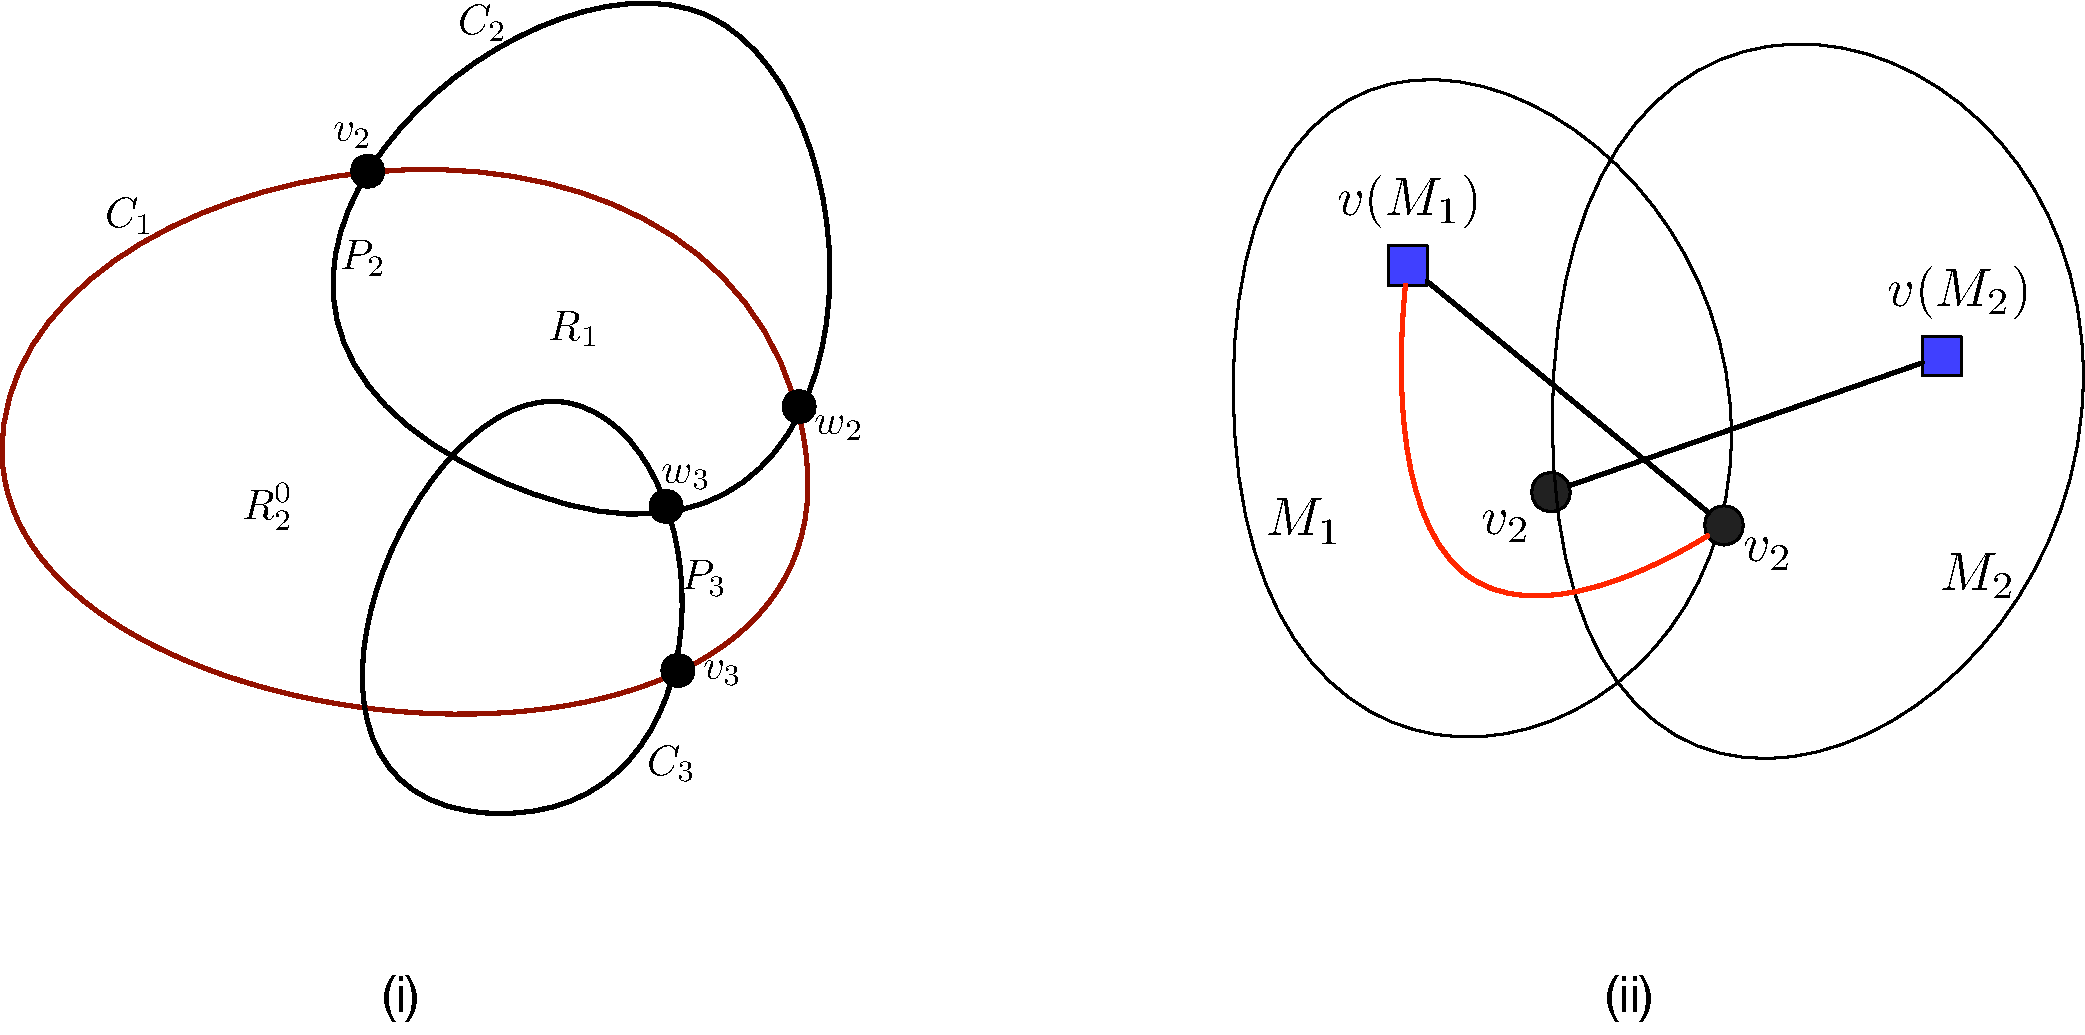
\includegraphics[width=.9\textwidth]{crossings.pdf}
\end{center}
\caption{\label{fig:crossings}Figure (i) illustrates crossing even
  cycles as discussed in Theorem \ref{1cross}. Figure (ii) illustrates
  the fact that
  the debit graph for our oracle is planar.}
\end{figure}

\begin{definition}
We say that cycles $A_1$ and $A_2$ {\em cross} if the set of common
faces is a proper subset of the faces of $A_1$ and $A_2$. E.g., in Figure \ref{fig:crossings}.(i), cycles $C_1$ and $C_2$ cross.
\end{definition}

We are now ready to show that face minimal cycles can not cross
arbitrarily. 

\begin{theorem}\label{1cross}
Each face minimal even cycle crosses at most  other  cycle.
\end{theorem}
\begin{proof}
Suppose that a face minimal even cycle $C_1$ crosses 2 other  cycles $C_2$, $C_3$.
Let $P_2$ be a subpath of $C_2$ s.t. the internal nodes of $P_2$ are in the interior of $C_1$, and the endpoints of $P_2$ are on $C_1$. Clearly, $P_2$ divides the interior of $C_1$ into two regions, $R_1$ and $R^0_2$. Suppose, w.l.o.g., that $C_3$ intersects the interior of $R^0_2$. Let $P_3$ be a subpath of $C_3$ such that its internal nodes lie in the interior of $R^0_2$, and its endpoints lie on the boundary of $R^0_2$. Hence, $P_3$ subdivides $R^0_2$ into $R_2$ and $R_3$.

Now note that the sum of the lengths of $R_1$, $R_2$, and $R_3$ equals $|C_1| +2(|P_2|+|P_3|)$, an even number by assumption. Hence, one of the $R_i$ must be an even cycle, contradicting the face-minimality of $C_1$. (see Figure \ref{fig:crossings}.(i) )
\end{proof}

An immediate consequence of the above theorem is that our debit graph
is planar. 

\begin{cor}
The debit graph for our oracle is planar.
\end{cor}
\begin{proof}
As in \cite{GW98} given the planar embedding of our graph $G$,  we draw (that is, we embed in the plane) our  debit graph  by placing a  node  $v(M)$ representing cycle $M$  in the interior of the region bounded by $M$  in $G$   and draw the edges $(v(M),h) $  of our debit graph by drawing an edge from  $v_M$ to node $h$  in $G$. 

In this drawing the only potential pairs of crossing edges are of the
form $ (v(M_1),h_1)$, $(v(M_2),h_2)$ where $M_1$ and $M_2$ are two
crossing even cycles (see Figure \ref{fig:crossings}.(ii)). However, since (by
Theorem \ref{1cross}) each face minimal even cycle crosses at most one
other face minimal even cycle. For such a crossing pair, we can {\em
  detour} (see Figure \ref{fig:crossings}.(ii)) our edges so they don't cross.
\end{proof}

Next we prove our key theorem where we show that, for a minimal hitting set, we may choose a family of witness cycles whose pairwise crossings are very restricted.  

\begin{definition}
Let us call a pairwise distinct triple $A_1, A_2, A_3 \in \mathcal{A}$ with $A_2, A_3$ both crossing $A_1$  \emph{nice}  
%s.t. $A_2$ and $A_3$ cross $A_1$, we must have that 
if (i) $A_2$ and $A_3$ are laminar, and (ii) $A_2$ and $A_3$ either differ in the interior of $A_1$, or they differ on the exterior of $A_1$ (but not both).
Formally, there are paths $Q,Q_2,Q_3$ $Q \subset A_2 \cap A_3 $ $ Q_2 \subset A_2 $, $Q_3 \subset A_3 $ whose interior does not intersect $A_1$. We then have that $A_i = Q \cup R_i \cup T_i \cup Q_i$ for $i=2,3$ where $R_i, T_i$ are subpaths of $A_1$ connecting $Q$ to $Q_i$.   
Let us call $\mathcal{A}$ nice if all $A_1,A_2,A_3 \in \mathcal{A}$ (pairwise distinct) are nice.  Let us consider 2 witness cycles $A_2, A_3$ to be equivalent if $A_1, A_2, A_3$ is a nice triple for some $A_1 \in \mathcal{A}$ and let us call the equivalence classes bunches.
\end{definition}

\begin{theorem} \label{laminar witness}
We may choose a nice family $\mathcal{A}$ of  (even) witness cycles and further no cycle of $\mathcal{M}$ crosses 2 cycles of $\mathcal{A}$.
\end{theorem} 
%Not quite right portion of path inside $A_1$ is confined to have the same endpoints, but can travel on $A_1$ before
\begin{proof}
First let us prove that a cycle of $M \in \mathcal{M} $ cannot cross 2 cycles $A_1 , A_2$ of $\mathcal{A}  $. The proof is basically the same as the proof of theorem \ref{1cross}. Let $P_1$ 
%(resp $P_2$) 
be a subpath of $A_1$ 
%(resp $A_2$) 
lying in the region bounded by $M$ s.t. the internal nodes of $P_1$ are in the interior of $M$ and the endpoints of $P_1$ are on $M$. $P_1$ path divides $M$ into two regions $M_1, M^0_2 $. W.l.o.g.,  $A_2$ intersects the interior of $M^0_2$. Let $P_2$ be a subpath of $A_2$ such that its internal nodes lie in the interior of $M^0_2$, and its endpoints lie on the boundary of $M^0_2$.  $P_2$ divides $M^0_2$ into 2 regions, which we call $M_2$ and $M_3$. Note that the sum of the lengths of $M_1$, $M_2$, and $M_3$ equals $|M| +2(|P_1|+|P_2|)$, which is even. So one of the $M_i$ is even contradicting face-minimality of $M$.\\
% Let $v_1 ,  w_1$ (resp $v_2, w_2$ ) be the end points of  $P_1$ (resp $P_2$) , then $v_1, w_1$ (resp  $v_2 , w_2$) split M into portions of the same parity.  If $P_1, P_2$ do not have any vertices in common then we may talk about the 3 regions that $P_1, P_2$ divides M into, then since the length of the boundaries of all 3 regions is $| M | +2( |P_1|+|P_2|)$ one of the regions must have even boundary contradiction. Otherwise let M' be one of the regions that $P_2$ divides M into (and contains an edge of $P_1$ in it's interior) and let $P_1'$ be the portion of $P_1$ that  stays in M' the consider the region $M \backslash M'$ and the two regions of M' divided by $P_1$' these sum up to $|M|+2(|P_2|+ |P_1'|)$  so one of these cycles is even.  \\
%
Next we introduce the uncrossing algorithm of \cite{GW98} on our witness cycles. % that is the 2 uncrossed cycles outputted by their algorithm are both even,  we will do so. 
\begin{definition}\label{uncrossing} \cite{GW98}
For  a set of witness cycles $ \mathcal{A} $ any two even cycles $A_1, A_2 \in \mathcal{A}$  that cross, we define the uncrossing operation: Let  $P_1, P_2 ,..., P_l ,Q_1, Q_2, .., Q_l$ be a series of internally disjoint paths such that $P_i$ (resp $Q_i$ )  are subpaths of $A_1$ (resp $A_2$)  for each $i$,  $P_i$ has the same endpoints as  $Q_i$  and , all $P_i$ (resp $Q_i$) lies in the interior of the region bounded by $A_2$ (resp $A_1$  ).  (Put simply $A_1 , A_2 $ cross each other at $P_i, Q_i $ see figures \ref{defcross} \ref{defcross2}. ) If 
% it is possible to ``switch" any of the $P_i$ with $Q_i$, that is
 for some $ S\subset [l] $ , if both of  $ A'_1 := A_1 \cup  (\cup_{i \in S}  Q_i ) \backslash (\cup_{i \in S}  P_i ) ,  \ \ \ A'_2 :=  A_2 \cup  (\cup_{i \in S}  P_i ) \backslash (\cup_{i \in S}  Q_i )  $  are even, and contain exactly one hit node then replace $A_1, A_2$ with $A'_1, A'_2 $  in $\mathcal{A}  $, that is we ``uncross" the specified $P_i, Q_i$. (See figure \ref{defcross}. )  Otherwise, if for some $i,$  $P_i \cup Q_i \in \mathcal{C}  $ is even, and contains exactly one hit node and there is an even cycle $C$ in $ (A_1 \cup A_2 \backslash P_i ) \backslash Q_i $ containing exactly one hit node, define  $ A'_1=P_i \cup Q_i ,   \ \ \ A'_2=C$. (See figure \ref{defcross2}. )   Replace $A_1, A_2 $   by $A'_1, A'_2 $   in  $\mathcal{A} $. (Otherwise we will say that $A_1, A_2$ cannot be uncrossed and the operation does nothing.) 
 % We will refer to this operation as our uncrossing algorithm. 
 
\begin{figure}[H]
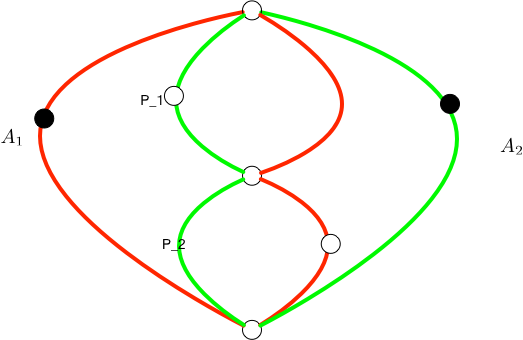
\includegraphics[scale=0.28]{CrossingCycle1.png}    \hspace{2cm}
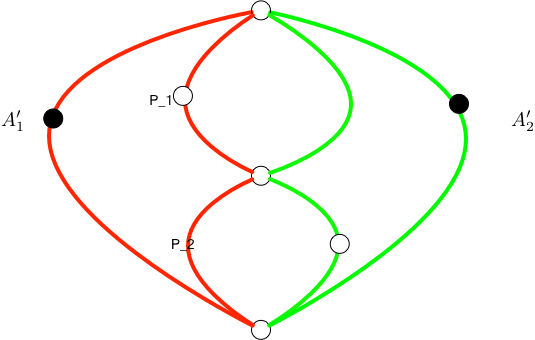
\includegraphics[scale=0.25]{Uncrossed1.png} 
\caption{ Example of uncrossing with $ A'_1 := A_1 \cup  (\cup_{i \in S}  Q_i ) \backslash (\cup_{i \in S}  P_i ) ,  \ \ \ A'_2 :=  A_2 \cup  (\cup_{i \in S}  P_i ) \backslash (\cup_{i \in S}  Q_i )  $  }
\label{defcross}
\end{figure}  %\\  
\begin{figure}
  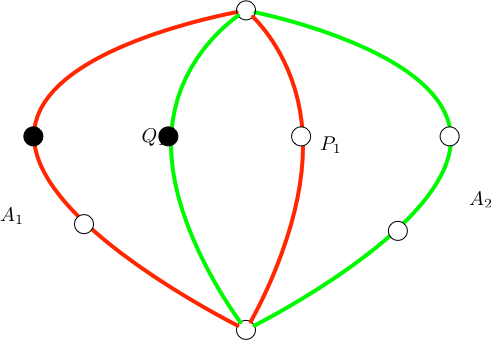
\includegraphics[scale=0.25]{CrossingCycle2.png}  \hspace{2cm}
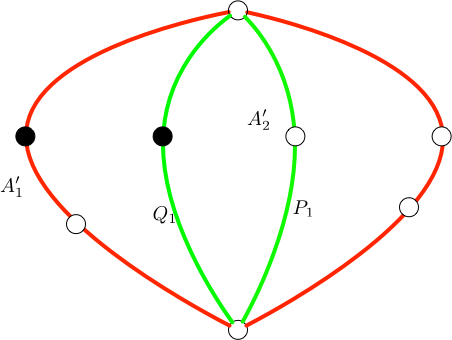
\includegraphics[scale=0.25]{Uncrossed2.png} 
\caption{ Example of uncrossing  with   $ A'_1=P_i \cup Q_i ,   \ \ \ A'_2=C$  } 
\label{defcross2}
\end{figure}
\end{definition}   
%Let us also define another uncrossing procedure,  
One can adapt the proof of lemma 4.2 in \cite{GW98} to show  that this kind of uncrossing action will eventually terminate. 
%and that it terminates with a set $\mathcal{A}$ with the fewest number of crossing pairs.  (That is the set $ | (A_1, A_2) \in \mathcal{A} \times  \mathcal{A}   \ \ \ A_1 \ \text{crosses} \ A_2   |  $ ) 
Further the uncrossing action does not increase the number of crossing pairs. ($ | (A_1, A_2) \in \mathcal{A} \times  \mathcal{A}   \ \ \ A_1 \ \ \text{crosses} \ \ A_2   |  $)
Thus starting with any set of witness cycles $\mathcal{A}'$, with the fewest number of crossing pairs,  using repeated applications of the uncrossing algorithm in definition \ref{uncrossing}, we can construct a set of witness cycles $ \mathcal{A} $, such that the uncrossing procedure of definition \ref{uncrossing}  can not be applied to any two cycles of $\mathcal{A}$ and also has the fewest number of crossing pairs. \\
Let us also introduce another uncrossing procedure 
\begin{definition}\label{uncrossing2}
If  $A_1, A_2$ cross and  $A_2$ consists of internally disjoint paths $Q,   R_1, P_1, R_2, P_2 ..,  P_l, R_l$  in that order with  $P_i,$  lies outside $A_1$  $ R_i$ lie on $A_1$ $Q$ lies inside $A_1$ for each $P_i,$ let  $B_i$ be the portion of $A_1$ connecting the endpoints of $P_i$ such that $P_i \cup B_i$ does not contain $A_1$ if it is possible to replace a subset of $P_i$ with $B_i$ to obtain an even witness cycle $A'_2$, and replacing $A_2$ with $A'_2$ in $\mathcal{A} $  does not increase the number of pairwise crossing cycles,  we do so. 
\begin{figure}
        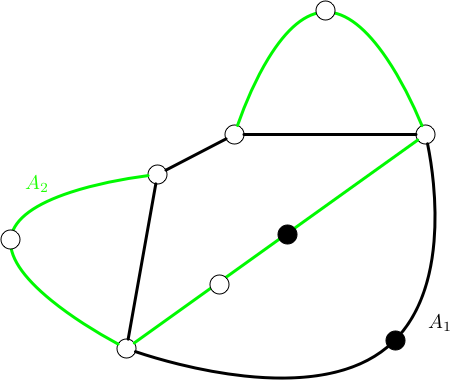
\includegraphics[scale=0.3]{uncrossing2.png}
      % \label{fig:my_label}
\end{figure}
\end{definition}

%(We henceforth assume it is not possible to uncross two witness cycles in  $ \mathcal{A} $.)  
%
\begin{lemma}\label{singlecross}
Let $A_1$ , $A_2$  be two crossing witness cycles. Then there does not exist 2 subpaths $ P_1,  P_2 $ of $ A_2  $  lying in the region bounded  by $A_1$,  (in our embedding of G in the plane) such that $ P_1 , P_2  $ are internally disjoint and each intersects  $A_1$   at their endpoints
%where $ a_i, b_i $ are the endpoints of $P_i$
, put simply, $A_2$ does not cross $A_1$ twice. (see figure \ref{doublecross} )  Further if $Q_1$ is a subpath of $A_2$ with endpoints $a_1,b_1$ on $A_2$  internally disjoint from $A_1$, %then  one such crossing 
then $Q_1$ has different parity than the paths between $a_1, b_1 $ in $A_1$. %  where $ a_1, b_1 $ are the endpoints of $P_1$. 
\begin{figure}[h]
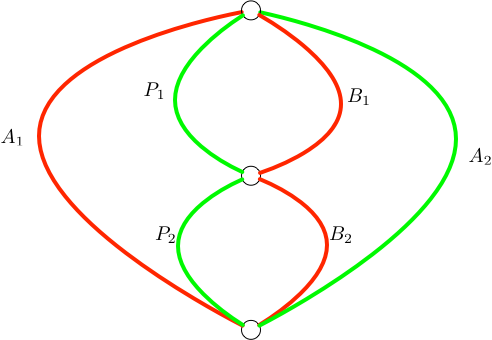
\includegraphics[scale=0.2]{DoubleCross.png}
\caption{}
\label{doublecross}
\end{figure}
\end{lemma}  

\begin{proof}
First suppose for a contradiction that $P_1 , P_2$ are two such paths, choose $P_1 , P_2 $  so that  there is  a path in $A_1$  internally disjoint from $A_2$   connecting an endpoint $a_1 $ of $P_1 $  with an endpoint  $b_2 $ of $ P_2 $. (That is $P_1, P_2$ are two ``consecutive" crossings ) Choose paths $B_1, B_2  \subset A_1$    internally disjoint connecting the endpoints of $P_1, P_2$ respectively. (see figure \ref{doublecross} )  % Note  $ B_1 \cap B_2 \subset \{ a_1, b_1 \}$  
%and let us choose $B_1, B_2$ shortest possible and  let us choose $P_1, P_2$ so the sum of the lengths of $B_1 , B_2$ is shortest.  Thus $ B_i \subset  A_2 \backslash \{ a_i, b_i \}$  
Now we may uncross either $P_1, B_1$ , $P_2, B_2$  or both  unless $P_1,B_1$  or $P_2, B_2$ has exactly one hit node. WLOG $P_1$ contains the hit node of $A_2$.  \\
 If  $P_2, B_2$ does not contain a hit node.  In this case, $P_2 , B_2$ must be of different parity. (otherwise $P_2 \cup B_2$ is an even cycle not hit) Thus the cycles $ (A_2 \backslash P_1) \cup  B_1 , \ \ \ (  (A_2 \backslash P_1 ) \cup  B_1 \backslash P_2 ) \cup B_2 $ are of different parity, so one must be even, but neither contains a hit node contradiction.  (See figure \ref{doublecrosscontradiction} )
 \begin{figure}[h]
           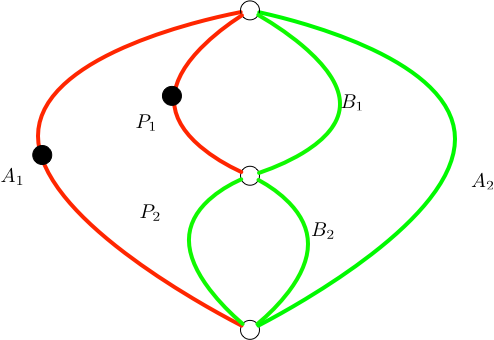
\includegraphics[scale=0.3]{DoubleCrossContradiction}  
           \caption{One of the green cycles is even and not hit.}
     \label{doublecrosscontradiction}
  \end{figure}
Thus the hit node of $A_1$ lies on $B_2$.
%In the same reasoning as above if there are two paths $Q_1, Q_2$   with $Q_i \subset A_i \backslash ( P_i \backslash a_i \backs lash  b_i )$ between 2 vertices $ u',v' \in A_1 \cap A_2 $, then choosing $ Q_1 $ to be of minimal distance, we may assume $Q_1 \cap Q_2 = \{u ',v' \} $ .  Since $Q_1 \cup Q_2 $ does not contain a hit node, $Q_1, Q_2$ are of opposite parity, thus one of $(A_2 \backslash P_1) \cup  B_1, (( (A_2 \backslash P_1) \cup  B_1 ) \backslash Q_2) \cup Q_1 $ is even but has not hitting node contradiction.  \\
If the closed walk  $ W:= (( A_1 \backslash B_1 ) \backslash B_2 )   \Delta ( A_2 \backslash P_1 ) \backslash P_2 )  $  is not a cycle, then it contains an odd cycle $C'$. Then $ (A_2 \cup B_1 \backslash P_1), (A_2 \cup B_1 \backslash P_1) \Delta C'$ are cycles of different parity, and are not hit, which is a contradiction. (see figure \ref{doublecrosscontradiction3})
\begin{figure}[h]
    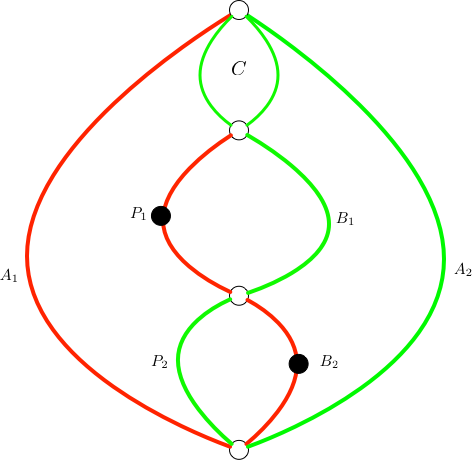
\includegraphics[scale=0.3]{DoubleCrossContradiction3.png}
    \caption{One of the green cycles is even and not hit which shows that $A_1,A_2$ cannot have ``too much intersection" so to speak.}
    \label{doublecrosscontradiction3}
\end{figure}
So $W$ is a cycle 
%and has length $ (( A_1 \backslash B_1 ) \backslash B_2 )   \Delta ( A_2 \backslash P_1 ) \backslash P_2 )  $ 
and has length $ |E(A_1) | + E(A_2) - |E(P_1 \cup B_1) | - |E(P_2 \cup B_2 ) |  -2 |E(A_1) \cup E(A_2) | $. As $|E(P_i \cup B_i) |$   are both odd we have this cycle is even, but not hit, a contradiction. (see figure \ref{doublecrosscontradicrtion2} )  
\begin{figure}[h]
    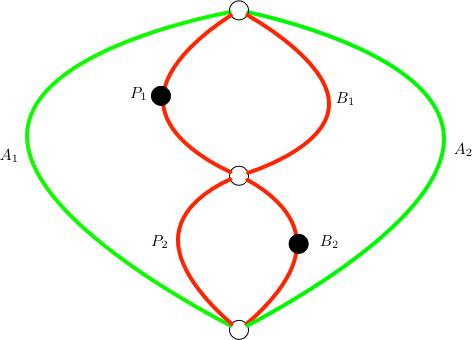
\includegraphics[scale=0.3]{DoubleCrossContradiction2}  
    \caption{Green cycle above is even and not hit.}
    \label{doublecrosscontradicrtion2}
\end{figure}

The last point (that $P_i , B_i$ are different parity) is because otherwise one of the hit nodes of $A_1, A_2$ must lie on the even cycle $P_i \cup B_i$.  W.l.o.g  the hit node of $A_2$ lies on $P_1$ then $A_2 \cup B_1 \backslash P_1$
%because otherwise $P_1$ splits $A_1$ into 2 even cycles and the hit node of $A_1$ cannot be on both, therefore the hit node of $A_2$ is an internal vertex of $P_1$ but then $A_2 \backslash (P_1 \backslash \{ a_1, b_1 \})$ combined with the path between $a_1, b_1$ in $A_1$ that does not contain a hit node of $A_1$ is an even cycle that is not hit contradiction.

\end{proof}

 Suppose for a contradiction, that for some $A_1, A_2 ,A_3 \in \mathcal{A}$,$A_1$ crosses $A_2 $ and $A_3$. Let us choose $A_1$ to bound the smallest region. let $P_2 , P_3$ be the portions of $A_2, A_3$ lying in $A_1$ let $u_2, v_2$ (resp    $u_3, v_3$ ) be the endpoints of $P_2$ resp $P_3$. 
 Let us define $p(A_i)$ to be the intersection of the outmost layer of $A_1 \cup A_i$ and $A_i$ and $b(A_i)$ to be the subpath of $A_1$ not in the outmost layer of $ p(A_i)  \cup A_1$. Choose $A_2 , A_3 $ with $b(A_2) $ minimal and of those with $b(A_3)$ minimal.
 %Define $B_2 $ (resp $B_3$ ) to be the subpath of $A_1$  lying in the region bounded by $A_2$. (resp $A_3$ ).
 % If the node of $A_i$ does not lie on $P_i$, define $P_i'=P_i$  otherwise, define $P_i'= A_i \backslash (P_i \backslash \{v_i, w_i \})$. (That is $P'_i$ is the subpath of $A_i$ with endpoints $u_i,v_i$ not containing the hit node of $A_i$) 
% We claim that  for i=2,3   it is possible to choose a subpath $ P'_i  $ of $A_i$ containing no hit node with endpoints $u'_i, v'_i$ such that for one choice of $B'_i$ is a subpath of $A_1$ between $u'_i, v'_i$.  $P'_i \cup B'_i$ is a cycle and does not cross $A_1$
% Where $B'_i$ is a subpath of $A_1$ between $u'_i, v'_i$. 

\begin{lemma}
If the hit node of $A_i$ lies on $P_i$, then the subpaths of $A_i$ connecting $P_i$ to $p(A_i)$ are part of $A_1$ (see figure \ref{P'def} ) and further $p(A_i)$ is internally disjoint from $A_1$.  
\end{lemma} 

\begin{proof}
Suppose for a contradiction that this is not true,  let $R$ be a subpath of a path connecting $P_i$ to $ p(A_i)  $ internally disjoint from $A_1$  and let $R'$ be the corresponding path in $b(A_i)$. Let $p_1(A_i)$ be the subpath of $p(A_i)$ internally disjoint from $b(A_i)$ such that $R$ is not in the outer layer of $p_1(A_i)$   By lemma \ref{singlecross}  $p_1(A_i) , q_1(A_i) $  and $R,R'$ have opposite parity. So $p_1(A_i) \cup (q_1(A_i) \backslash R') \cup R$ is an even cycle and thus the hit node of $A_1$ lies on $q_1(A_i) \backslash R' $. Note that $p_1(A_i) \cup (A_1 \backslash q_1(A_i)) , R \cup R'$ are both odd cycles with no hit node, and thus are not crossed by any cycle.  This and minimality of $b(A_i)$ means that replacing $A_i$ with $A'_i:= p_1(A_i) \cup (q_1(A_i) \backslash R') \cup R$ in $\mathcal{
A}$ leads to fewer pairwise crossings contradiction. 
Now we prove that $p(A_i)$ is internally disjoint from $A_1$ assume not, then let $p(A_i) = p_1(A_i) \cup r_1(A_i) \cup ... \cup p_j(A_i)$ where $p_l(A_i) $ are internally disjoint from $A_1$ and $r_{l}(A_i)$ is a subpath of $A_1$ connecting $p_l(A_i)$ to $p_{l+1}(A_i)$, let $T_l$ be the subpath of $A_1$ not one the outside layer of $A_1 \cup p_l(A_i) $ then by lemma \ref{singlecross}  $p_l(A_i) , T_l$ are different parity and thus replacing $p_1(A_i) , p_2(A_i)$ with $T_1, T_2$  via the uncrossing method of definition \ref{uncrossing2} yields a contradiction.
\end{proof}

 % \begin{lemma}
%Either $P_2 = P_3$ or both $P_2,P_3$ contain a hit node.
%\end{lemma} 
%\begin{proof}
%%Suppose not, w.l.o.g  $P_3$ contains no hit node by lemma \ref{singlecross} 
% \end{proof}

If $P_i$ does not contain a hit node, then set $P'_i=P_i$ otherwise, let $P'_i = p(A_i)$  %be the intersection of the outmost layer of $A_1 \cup A_i$ and $A_i$. 
If $P'_i = P_i$ define $B_i$ to be the portion of $A_1$ lying in $A_i$, otherwise define $B_i$ to be the portion of $A_1$ not lying in the outer layer of $ A_1 \cup P'_i$. (see figure \ref{P'def} )  Define $u_i ,v_i$ to be the endpoints of $B_i$
\begin{figure}
        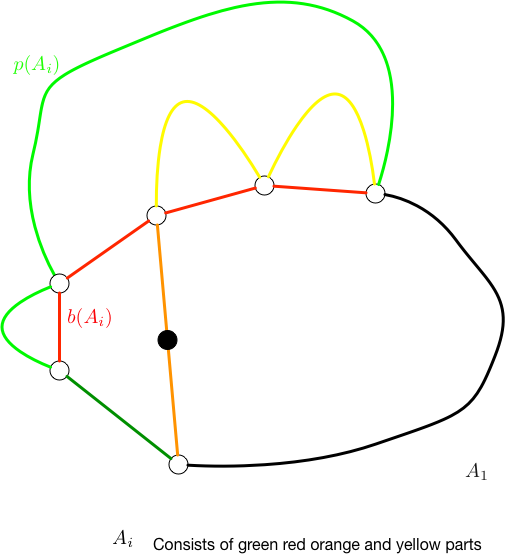
\includegraphics[scale=0.3]{p(A_i).png}
        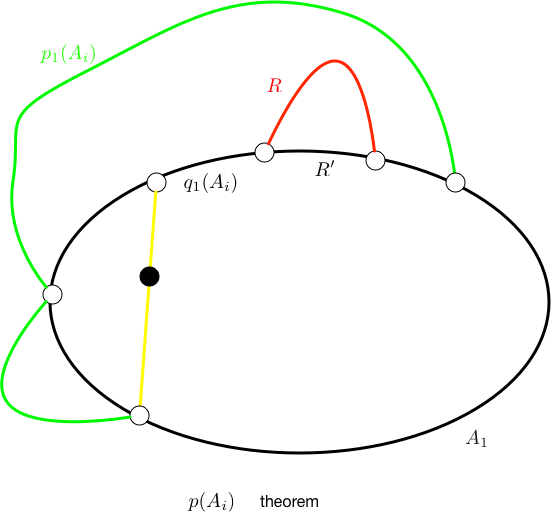
\includegraphics[scale=0.3]{p(A_i)thm.png}}
            %\caption{Caption}
    \label{P'def}
\end{figure}

% let $H$ be a maximal subpath of $A_2$ with $u_i$ on one end and $B_i$ is disjoint from the interior of any region bounded by a subgraph of subgraph of $A_1$ $ R_1, Q_1, .., R_l Q_l R_{l+1}$ be a series of paths such that

\begin{lemma}
$P'_2, P'_3$ are internally disjoint
\end{lemma}
\begin{proof}
\begin{figure}[h]
      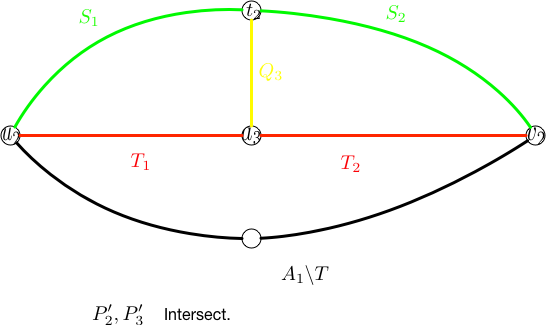
\includegraphics[scale=0.3]{P'_2P'_3intersect.png}
       \label{P'_2P'_3inter}
\end{figure}
Assume not, since $A_2,A_3$ is not nice, either, i) there is a subpath $Q_3$ of $P'_3$ connecting a node $a_3 \neq u_2, v_2$ on $A_1$ ($a_3$  will be $u_3$ or $v_3$ ) to an internal node $t_2$ on $P_2$, or ii) there is a subpath $R$ of $P'_3$ internally disjoint from $P'_2$ between 2 nodes $r,r'$ of $P'_2$. Consider case i) let $T$ be the subpath of $A_1$ connecting $u_2$ to $v_2$ with $a_3$ in the interior. Let $T_1$ be the subpath of $T$ from $u_2$ to $t_2$, and $T_2$ the subpath of $T$ from $t_2$ to $v_2$. Let $S_1$ be the subpath of $P'_2$ from $u_2$ to $t_2$ and $S_2$ the subpath of $P'_2$ from $t_2$ to $v_2$. (see figure \ref{P'_2P'_3inter} ) By lemma \ref{singlecross}  $S_1 \cup Q_3 \cup T_1 , S_2 \cup Q_3 \cup T_2$ are odd cycles, which means $S \cup T $ is even contradicting lemma \ref{singlecross}.  For case ii), let $R'$ be the corresponding path in $P'_2$ by lemma \ref{singlecross} $R',R$ have different parity. Since both $P'_2 , (P'_2 \backslash R' ) \cup R $ have no hit node, they have different parity than the corresponding path between the endpoints of $P'_2$ in $A_1$, which is a contradiction.
\end{proof}

Now we deal with the remaining case.
 \begin{lemma}\label{disjointP_i} 
 %Suppose $B_2, B_3$ are subpaths of $A_1$, $B_i$ connecting $u_i$ to $v_i$. 
 ( $P'_i, B_i $ as defined above ) It cannot be that  $P'_2, P'_3,  $ are internally disjoint (see figure \ref{disjointPi}   )% and  $B_2, B_3$ are either internally disjoint, or one is a subpath of the other
 . 
\begin{figure}
        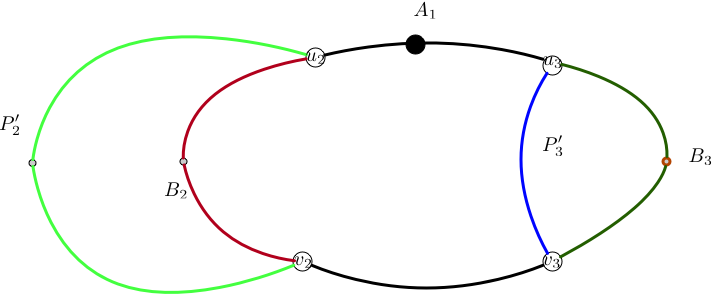
\includegraphics[scale=0.3]{DisjointP_i.png}
              % \caption{}
        \label{disjointPi}
   \end{figure}
 \end{lemma}
\begin{proof} 
First let us address the case that $B_2, B_3$ are either internally disjoint, or one is a subpath of the other. Let $u_i, v_i$ be the endpoints of $B_i$ such that $u_2, v_2, v_3, u_3$ appear on $A_1$ in that order. W.l.og.  $B_2$ does not strictly contain $B_3$ define $B'_2 =B'_2$ and $B'_3$ the subpath of $A_1$ connecting $u_3, v_3$ that is internally disjoint from $B'_2$.
Assume otherwise, since $P_2' , P_3' , B'_2 ,B'_3$ are internally disjoint,  $(A_1 \cup P'_2 \cup P'_3 ) \backslash (B'_3 \cup B'_2)$ is an even cycle. So the hit node of $A_1$ does not lie on $B'_2$ or $B'_3$.   %
%Letting $u_i, v_i$ be the ends of $P'_i$ 
%Let us denote by $C_i$ the subpath of $A_1$ from $u_i$ to $v_i$ not containing the hit node. 
We claim that for $i=2,3$ the cycle $ D_i:= (A_i \cup B'_i ) \backslash P_i$ does not cross any other cycle of $\mathcal{A}$.  Assume the contrary, that $D_i$ crosses $W \in \mathcal{A}$.  Let $W= W_1 \cup .. \cup W_t$ be a decomposition of $W$ into internally disjoint paths which are internally disjoint from $D_i$. W.l.o.g  $W_1$ does not contain  the hit node of $W$. Let $a,b$ be the endpoints of $W_1$ and let $P$ be a path between $a,b$ in $D_i$.  Then by Lemma \ref{singlecross}, $W_1 , P$ are different parity so $D_i \backslash P_i \cup W_1$ is an even cycle that is not hit contradiction.
%We claim $W$ does not cross $D_i$ twice, that is we can divide $W$ into two subpaths $W_1, W_2$  $W= W_1 \cup W_2 $ such that   $W_1 $  lies inside the region bounded by $D$ and $W_2$ lies outside the region bounded by $D$. Indeed if $W$ crossed $D_i$ twice then $W$ crosses either $A_1$ or $A_i$ twice which contradicts lemma \ref{singlecross}. Let  $W_j$ be the subpath of $W$ not containing the hit node, and let $D'_i$ be a sub path in $D_i$  between the two endpoints of $W_j$, then $D'_i$ has different parity from $W_j$. Now $ (D_i \cup W_j) \backslash D'_i $ is even and not hit contradiction.  \\ 
This proves that replacing $B'_i$ %or $A_1 \backslash C_i$ 
with $P'_i$ in $A_1$ for $i=2,3$ decreases the number of crossing pairs in $\mathcal{A}$. (that is $\mathcal{A} \cup (A_1 \cup P'_2 \cup P'_3 \backslash B'_2 \backslash B'_3 ) \backslash A_1  $ has fewer pairwise crossings which is a contradiction)
%If $B_2,B_3$ are internally disjoint, note one of $ A' :=  A_1 \cup P'_2 \backslash B_2 , A" :=  A_1 \cup P'_3 \backslash B_3 , A"'_1:=  A_1 \cup P'_2 \cup P'_3 \backslash (B_2 \cup B_3) ,   $ is even and  contains at most one hit node.
%If $B_2 \subset B_3 $ note one of $ A' :=  A_1 \cup P'_2 \backslash B_2 , A" :=  A_1 \cup P'_3 \backslash B_3 , A"'_1:= (A_1 \backslash B_3) \cup P_3 \cup P_2 \cup (B_3 \backslash B_2)$ is even and contains at most one hit node. In both cases replacing $A_1$ with $A'_1 , A"_1$ , or $A"'_1$  in $\mathcal{A}$ yields a family of witness cycles with fewer crossing pairs. This is a contradiction. (see figure \ref{disjointPicont} )  
%  in second case  $A_2$ gets uncrossed
\begin{figure}
    \centering
    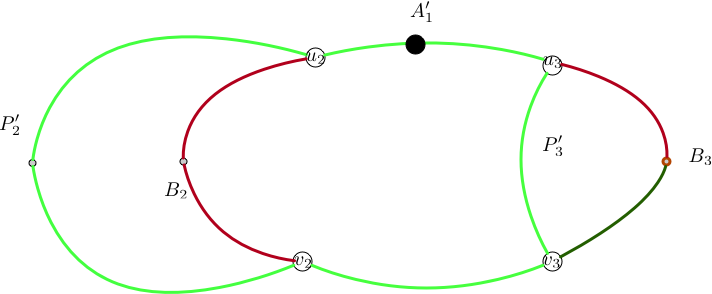
\includegraphics[scale=0.3]{DisjointP_iCont}
     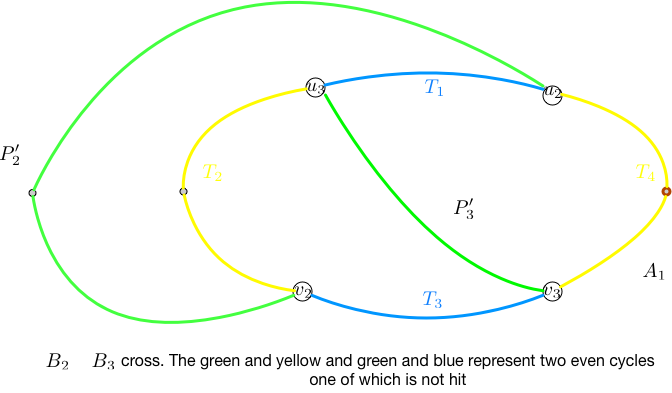
\includegraphics[scale=0.3]{DisjointP_icross.png}
    %\caption{}
    \label{disjointPicont}
\end{figure}
Now suppose that $ B_2 \backslash B_3 , B_3 \backslash B_2$ are both nonempty. Let $u_i, v_i$ be the endpoints of $ B_i $ so that $ u_2 , u_3 , v_2 , v_3 $  appear on $A_1$ in that order, and denote $ T_1, T_2, T_3, T_4 $ be the corresponding paths between the vertices in $A_1$ with $T_1$ the path between  Since $ B_2 \backslash B_3 , B_3 \backslash B_2 \neq \emptyset$, $ u_2 , u_3 , v_2 , v_3 $  are all distinct. By lemma \ref{singlecross}  $ P'_2 \cup T_2 \cup P'_3 \cup T_3, P'_2 \cup T_1 \cup P'_3 \cup T_4 $ are both even and the hit node of $A_1$ cannot lie on both contradiction. (figure \ref{disjointPicont} $B_2 ,B_3$ cross)
\end{proof}

%\begin{lemma}\label{}
%It cannot be the case that  %$P'_2, P'_3$ both lie outside $A_1$ and
%$B_2, B_3$ are either internally disjoint, or one is a subpath of the other. % (that is  they lie on the same subpath of $A_1$ that $u_3,v_3$ divides $A_1$ into )
%\end{lemma} 
%\begin{proof}
%Choose subpaths $B_2,B_3$ of  $A_1$ with  $B_i$ connecting $u_i$ to $v_i$ and $B_2,B_3$ internally disjoint.
\begin{figure}[h]
        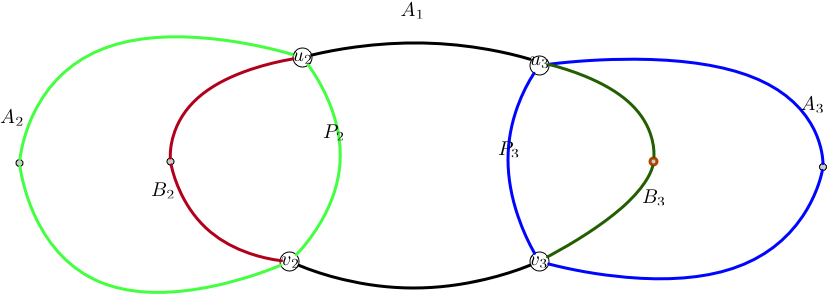
\includegraphics[scale=0.3]{Case1.png}
    \caption{Case 1)}
    %\label{Case1}
\end{figure} 
% By lemma \ref{singlecross}, $P_i$ must have the different parity  than $B_i$. 
%By lemma \ref{singlecross}  $ P'_i$ is internally disjoint 
%By lemma \ref{disjointP_i} $P_2', P_3'$ are not internally disjoint, then % $P_i'=A_i \backslash (P_i \backslash \{v_i, w_i \})$ , and
%Suppose for a contradiction, there are nodes $r,r'$ of $P'_3$ such that there is subpath $R_2$ of $P'_2$ connecting $r,r'$ different from the corresponding path in $P'_3$. Let $R_3$ be the subpath of $P'_3$ between r,r' in $P'_3$.  Then $R_2 , R_3 $ have different parity. W.l.o.g. the hit node of $A_1$ does not lies on $B_3$, then the cycles $ P'_3 \cup B_3 $ , $ ( P'_3  \backslash R_3 ) \cup B_3 \cup R_2 $ have different parity but no hit nodes, which is a contradiction. (see figure \ref{case1contr} )
%\begin{figure}[h]
 %      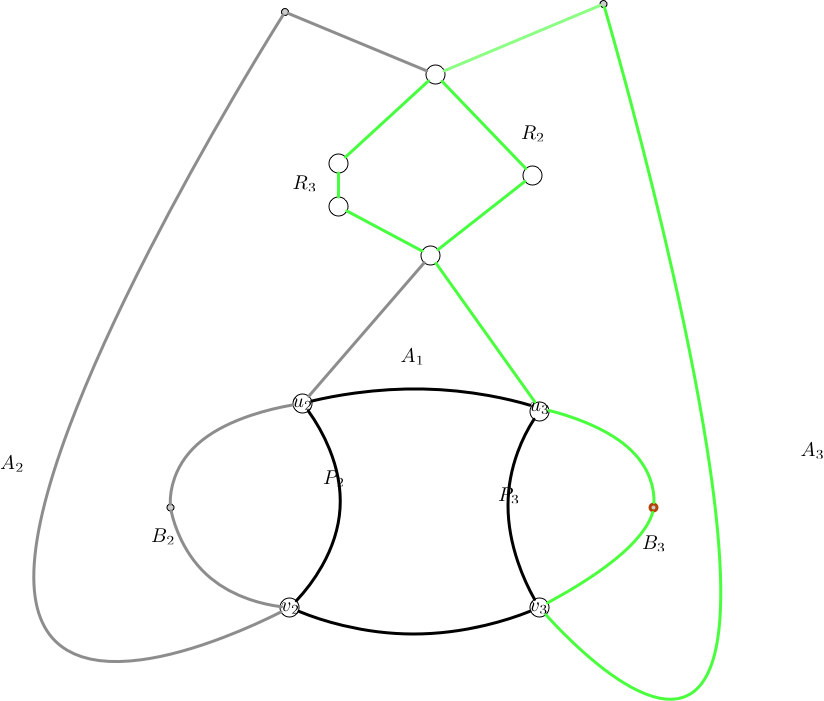
\includegraphics[scale=0.23]{Case1Contr.png}
  %  \caption{One of the green cycles is even and not hit}
   % \label{case1contr}
%  \end{figure}  
%Thus $ (P'_3 \Delta P'_2 ) \cup B_2\cup B_3 $ is an even cycle (parity follows because $P'_i , B_i $ are different parity) thus the hit node of $A_1$ lies on $B_2 \cup B_3$. W.l.o.g. it lies on $B_2$. (see figure \ref{case1contr2}  )
%\begin{figure}[h]     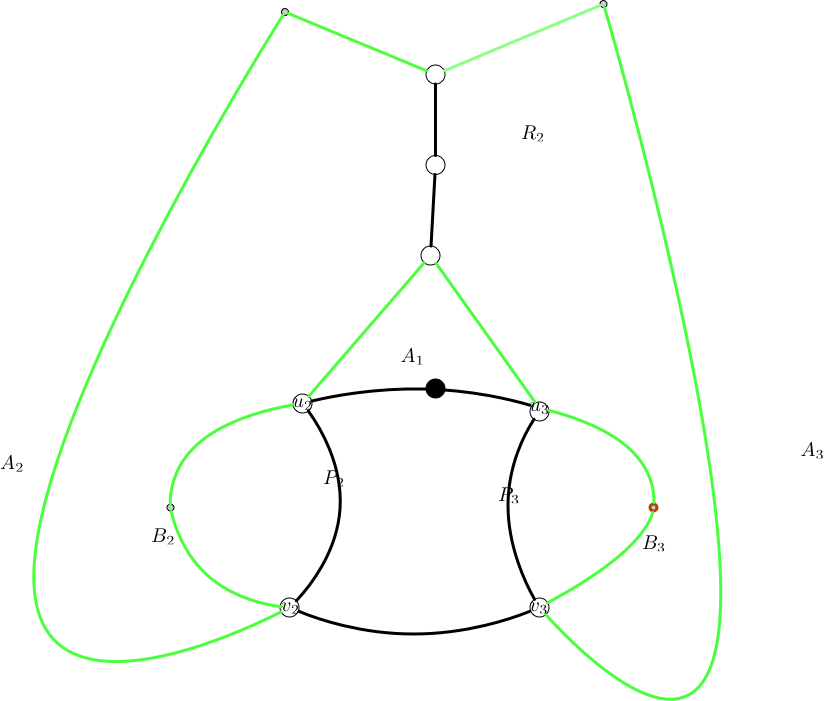
\includegraphics[scale=0.23]{Case1Contr2.png}      \caption{}     \label{case1contr2}
%\end{figure}
%Let $r$  be the first common vertex of $P'_2, P'_3$ and $r'$ be the last common vertex (when viewing $P'_i$ to go from $v_i$ to $u_i$  ) Denote by $F_i'$ the subpath of $P'_i$ from $v_i$ to $r$  and   $H'_i$ the subpath of $P'_i$ from $r'$ to $u_i$;  by $H$ the subpath of  $A_1$ from  $u_2$ to $u_3$  and $F$ the subpath of $A_1$ from $v_2$ to $v_3$ not hitting $u_2$. Now notice that the sum of the lengths of the cycles $F_2 \cup F_3 \cup F$ and $H_2 \cup H_3 \cup H$ is even and are not both trivial by assumption. Since the hit node of $A_1$ lies on $B_2$, both  $F_2 \cup F_3 \cup F$ , $H_2 \cup H_3 \cup H$  are odd so one of $ B_3 \cup P'_3 ,  B_3 \cup P'_3 \Delta (F_2 \cup F_3 \cup F) $ is even and not hit contradiction.


%\end{proof}
%We now deal with the final case.
%\begin{lemma}
%We cannot have $B_2 \backslash B_3 , B_3 \backslash B_2 \neq \emptyset$
%\end{lemma}
%\begin{proof}
%By a previous lemma $P'_2 , P'_3$ are not internally disjoint.  Let $Q_3$ be a 
% \end{proof}
 % We consider the following cases:\\

% Case 1)  $P_2$ , $P_3 $ are internally disjoint. 
%between $v_2, u_2 $ not hitting $P_3$ define $B_3$ analogously. 


%W.l.o.g   the hit node of 
%If the hit node of $A_1$ lies on $B_2 \cup B_3$, then $(A_1 \cup P'_2 \cup P'_3 ) \backslash $

%Then, replacing both $B_2$ with $P_2'$ and $B_3$ with $P_3'$  yields an even cycle so we can uncross $A_1$ from $A_2$ and $A_3$.  \\
%%
% case 1b)  suppose that the node of $A_1 $ lies on $B_2$ then if $P_3 , B_3$ have the same parity, uncross $A_1 , A_3$  (   If the node of $A_3$ does not lie on  $B_3$ then replace $P_3$ with $B_3$  otherwise, the cycle $P_3, B_3$ is even ) , since $B_3 \cup P_3'$ contains no hit nodes, $B_3, P_3'$ have different parities thus one of $P_2' \cup ( A_1 \backslash P_2 \backslash B_3 ) \cup P_3 , \ \ P_2' \cup ( A_1 \backslash P_2  ) $ is even but hits no other nodes contradiction. If the node of $A_2$ does not   otherwise .. actually this case might be problematic    edit should work because if this were the case the  cycle obtained from $A_1 $ by replacing by is even but this cannot be the case as all even cycles are hit. \\ 

%Case 2 $P_2,P_3$  intersect.  \\
%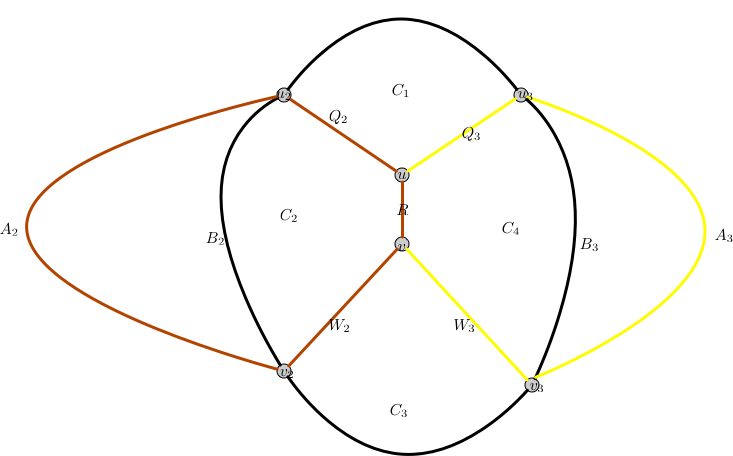
\includegraphics[scale=0.3]{Cross.png}
%Case 2 a)  $ u_2, v_2 $ (can be thought of to ) lie on the same side of $v_3, u_3 $, then let $P_2, P_3 $ intersect at $u,v$ that is there exists   a path  $ R \subset P_i$  connecting $u, v$. Again choose subpaths $B_2,B_3$ of  $A_1$ with  $B_i$ connecting $u_i$ to $v_i$ and $B_2,B_3$ internally disjoint. 
%By lemma \ref{disjointP_i} one of ($=2,3$) $A_i \backslash P_i$ contains a hit node.
%Like in case 1 if $ A_i \backslash  P_i $ contains no hit nodes for i=2,3  , then  w.l.o.g. $B_3$  contains no hit node  so  $(A_3 \backslash P_3 )  \cup B_3 $ is odd
%  note$ (A_1 \backslash B_2 ) \cup (A_2 \backslash  P_2 )  ,  \ \ ((A_1 \backslash B_2)  \backslash B_3 ) \cup (A_2 \backslash  P_2 ) \cup (A_3 \backslash  P_3 ) $  are of different parity and contains no hit node.   If $(A_1 \backslash B_2 ) \cup (A_2 \backslash  P_2 ) $ is even  contradiction otherwise 
%Define $Q_i$ to be the path from u to $u_i$,  and  $W_i$ the path from $v$ to $v_i$    so $  (A_2 \backslash P_2  ) \cup W_2 \cup W_3 \cup Q_2 \cup Q_3 \cup B_3   , \ \ (A_2 \backslash P_2  ) \cup W_2 \cup W_3 \cup Q_2 \cup Q_3 \cup (A_3 \backslash B_3 ) $ . 
%are of different parity and contain no hit node, which is a contradiction.
%and  $K_i$ the path from  $u_i$ to $v_i$   
%this is this implies either a direct contradiction
% or that $A_1$ can be uncrossed which is also a contradiction.  
%Thus w.l.o.g.  $P_2 $ contains no hit node denote by $R$ the path from $u$ to $v$ in $P_2$ .
% WLOG R is part of $P_2$ which contains no hit node. Denote by $ Q_i $ the portion of $P_i$ from $u_i$ to u and $W_i$ the portion of $P_i$ from v to $v_i $ . Let $R'$ be  the  path from u to v in $P_3$.   
%Let $ C_1 , C_2, C_3, C_4 $ be the faces of  $A_1 \cup P_2 \cup Q_3 \cup W_3 $ in counter clockwise order with  $C_2$ the portion bounded by $B_2, P_2$ . Since R is part of $P_2$  ,  $C_2$ is odd ( lemma \ref{singlecross}) so either  $ C_1 $  and $   C_4 \Delta  C_2  \Delta C_3 $  are both even, or  $C_1 \Delta C_2$  and $C_3  \Delta  C_4 $ are both even hence the hit node of $A_3$ lies on $Q_3 \cup W_3 $.   WLOG the hit node of $A_3$ lies on $Q_3$.  
%If $C_3$ is even, then the hit node of $A_1$ lies on $C_3$ and hence $  (  A_1 \Delta C_4    \Delta C_1  ) \cup A_3 , \  (  A_1 \Delta C_3) \cup A_3    $  have different parity and are not hit contradiction.  
%If the hit node of $A_1$ lies on  $C_3$  then $A_3 \cup (A_1 \Delta C_3 \Delta C_2 ) $  , $A_3 \cup (A_1 \Delta C_3  ) $    are different parity and not hit  if the hit node of $A_1 $ lies on $C_2$ then $C_3$ is odd and  $A_3 \cup (A_1 \Delta C_2 \Delta C_3 )   , \  \ A_3 \cup (A_1 \Delta C_2  )  $  are different parity and not hit contradiction. \\
%edit  should be that  either   $C_1 \Delta C_2 , C_1$  is even and  either $C_1 \Delta C_2 , C_1$  is even  and the node of $A_3$ cannot hit both.
 %   \indent	Case 2b) $u_2, v_2$ lie on different sides of $v_3, u_3 $.   WLOG $u_2$ lies inside $A_3$ and $v_2$ lies outside $A_2$.   Let $u$  be the first vertex $ P_3$ intersects $P_2 $ and $v$ be the last (when considering $P_3$ to go from $u_3$ to $v_3$ ).
%
% LOG $u$ lies between  $u_2$ and $v$ in $P_2$. Denote by $R_i$ the portion of $P_i$ between $u_i $ and u and $Q_i$ the  portion of $P_i$ from v  to $v_i$.  WLOG suppose that $v_2$ lies inside $A_3$  let w be the first vertex of $A_3$ in the path  from $v_2$ to $u_2$ in $A_2 \backslash P_2$. Let $L_2 , L_3$ be the paths from $ v_2$ to w and $u_3$ to w respectively.  Let $T_i $ be the path from u to v in $P_i$ we claim $T_3= T_2 $. Assume for a contradiction let $u' ,v'$ be nodes on $T_2 $  such that the path $T_3'$ in $T_3$ between $u',v'$ in $T_3$ is internally disjoint from $T_2 $ let $T_2'$ be the path from $u', v'$  in $P_2$. \\
%First if $T_2', T_3'$ have the same parity, then one of them $T_j$ contains a hit node, but then $ ( A_j \backslash T_j )  \cup T_l$  where $l \in \{ 2,3 \} \backslash j$  is an  even cycle so $T_l$ contains a hit node as well. If $B_2 \backslash B_3 \cup R_3 \cup Q_2$ is even, then so is $ ( A_1 \backslash  (B_2 \backslash B_3)  ) \cup R_3 \cup Q_2$  and the hit node of $A_1$ cannot hit both.
%Thus $B_2 \backslash B_3 \cup R_3 \cup Q_2$ is odd. Then $ A_2 \backslash (P_2 \cup L_2 ) \cup L_3 \cup R_3 \cup Q_2$ is of different parity as $ A_2 \backslash (P_2 \cup L_2 ) \cup L_3 \cup ( B_2 \backslash B_3 ),  A_2 \backslash (P_2 \cup L_2 ) \cup L_3 \cup (A_2 \backslash ( B_2 \backslash B_3 )  ), $ and not both of these can contain the hit node of $A_1$ contradiction.  \\
% Thus $T_2', T_3'$ have different parity if one of these WLOG $T_2$ contains a hit node, then if $T_3$ does not contain a hit node, then  $Q_2 \cup T_3 \cup R_2 \cup B_2 $   or  $Q_2 \cup T_3 \cup R_2 \cup ( A_1 \backslash B_2 ) $  is an even cycle with no hit node contradiction, otherwise like in the above paragraphs, $B_2 \backslash B_3 \cup R_3 \cup Q_2$ is odd,  as $ (A_2 \backslash (P_2 \cup L_2 )  ) \cup L_3 \cup ( B_2 \backslash B_3 ),  (A_2 \backslash (P_2 \cup L_2 ) ) \cup L_3 \cup (A_2 \backslash ( B_2 \backslash B_3 )  ), $ are different parity and not both of these can contain the hit node of $A_1$ contradiction. One of each of the following pairs of cycles   $ (B_2 \cap B_3 ) \cup R_3 \cup R_3 \cup T_i  ; \ \ \ ( A_1 \backslash (B_2 \cap B_3 ) ) \cup R_3 \cup R_3 \cup T_i  ; \ \ \   (A_1 \backslash  (B_2 \cup B_3 ) ) \cup Q_2 \cup Q_3 \cup T_i ; \ \ \  (B_2 \cup B_3 )  \cup Q_2 \cup Q_3 \cup T_i ; \ \ \ (A_3 \backslash T_3) \cup T_i ; \ \ (A_2 \backslash T_2) \cup T_i $ 
  % this implies (*) one of $R_2, R_3$ is hit, one of $Q_2, Q_3$ is hit, one of $ Q_i, R_i$ is hit.  \\
  % If $ (A_2 \backslash  L_2) \cup  L_3 \cup (B_2 \backslash B_3) $ is even, so is $ (A_2 \backslash  L_2) \cup  L_3 \cup (  A_1 \backslash ( B_2 \backslash B_3  ) ) $ and not both cycles can be hit while satisfying (*) so   $ (A_2 \backslash  L_2) \cup  L_3 \cup (B_2 \backslash B_3) $ (and likewise  $ (A_3 \backslash  L_3) \cup  L_2 \cup (B_3 \backslash B_2) $ )  is odd. Then for $i=2,3$  , $l= \{2,3 \} \backslash l $ either $  A_i \backslash L_i \cup L_j \cup R_j  \cup Q_i $ is even, or both $( A_1 \backslash ( B_i \backslash B_l  ) ) \cup  R_l \cup Q_i ,  \ \ ( B_i \backslash B_l   ) \cup  R_l \cup Q_i $ are, or that one of $Q_2 ,R_3$ and one of $Q_3 , R_2 $ is hit, combining with (*) we see this is not possible.  \\
   % Let $C_i$ be as in the diagram below,if $C_1$ is odd, then $C_2, C_3 , C_4 $ are all even, (lemma \ref{singlecross} ) so each contains a hit node,  then replacing $A_1$ with   $C_4$ uncrosses $A_1$ contradiction , if $C_1$ is even, then  
 % so is $C_5$  and $C_4, C_3, C_2 $ are odd, so   $ ( A_2 \backslash (L_2 \cup P_2) )  \cup L_3 \cup (B_3 \backslash B_2 ) ,  ( A_3 \backslash (L_3\cup P_3) )  \cup L_2 \cup (B_2 \backslash B_3 )   $  are even cycles, thus 2 of the hit nodes of $ A_1, A_2, A_3$  lie on these cycles and only one can lie on $C_5$ so replace $A_1$ by $C_5$ .
% $, A_1 \backslash C_4 \ A_1 \backslash  C_1 $  thus $ R_i, Q_{  \{ 2,3 \} \backslash i  }  $  for i=2 or 3  then for $l \in \{ 2,3 \} \backslash i $  $ (A_i \backslash L_i )  \cup  L_l \cup R_l \cup Q_l   $ is even and not hit contradiction .
   %$C_3, C_4$ are odd and  $C_5$ is even and one of $C_1, C_5 $ and contains only one hit node, if it is the hit node of $A_1$ we can uncross contradiction, otherwise two hit nodes lie on $ R_i, Q_{  \{ 2,3 \} \backslash i  }  $  for i=2 or 3 and then for $l \in \{ 2,3 \} \backslash i $  $ (A_i \backslash L_i )  \cup    $
   %\begin{wrapfigure}{r}{0.5\textwidth} 
   %\begin{center}
   %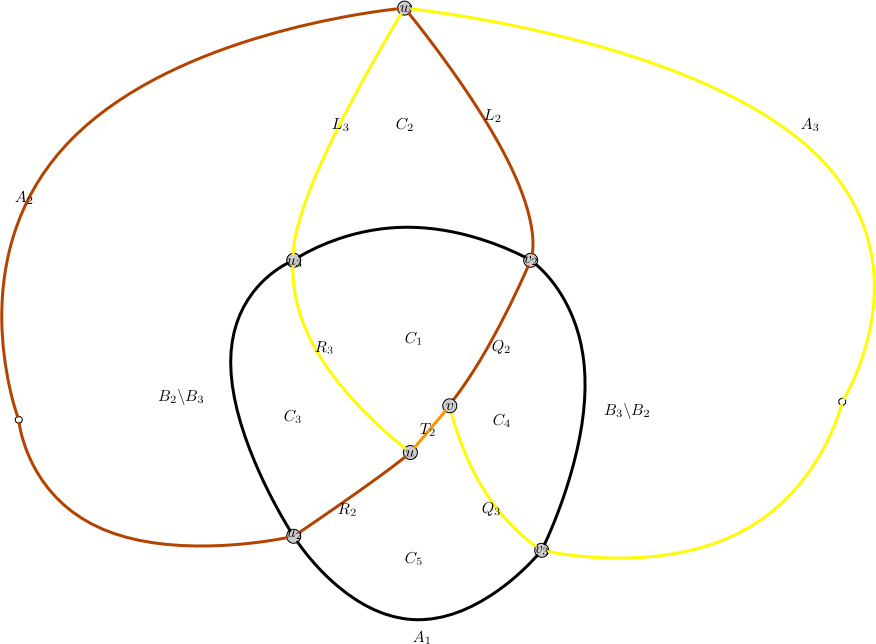
\includegraphics[scale=0.3]{cross2.png} 
    %  \end{center}
% \caption{Diagram for case 2b)    $u_2, v_2$ lie on different sides of $v_3, u_3 $  }
%  \end{wrapfigure}

% vertices $u_1, w_1 , u_2 , w_2$ and paths $ U_1, U_2 , W_1 W_2$
\end{proof} 
%%%  
%?? \begin{theorem} \label{laminar witness}
%We may choose a family $\mathcal{A}$ of witness cycles such that each witness cycle crosses at most two other witness cycle and each  cycle of $ \mathcal{M} $ crosses at most one other cycle of $ \mathcal{A} $
% \end{theorem}    
% \begin{proof}

\begin{lemma} \label{laminar bunch}
Cycles in bunches are laminar.
\end{lemma}
\begin{proof}
%For 2 witness cycles $B, C$ of a bunch, let us define the distance between $B,C$  $d(B,C)$ to be the minimum m such that for some $B_0, B_1 ,.., B_m$ in our bunch $B=B_1 , C= B_m$  we have that $A, B_i, B_{i+1}$ is a nice triple for some  $A \in \mathcal{A}$.   
If $B,C $ are cycles in a bunch, then they share a non empty path $Q$  write $B = Q \cup B_1 \cup B_2 \cup .. \cup B_m$  where $B_i$ is internally disjoint from $C$ if $B,C$ cross them $m>2$ as $B \backslash Q$ needs a subpath that lies inside that lies inside the region bounded by C and a subpath that lies outside the region bounded by C.  Let $C_i$ be the path in $C \backslash Q$ between the endpoints. This violates lemma \ref{singlecross}.
\end{proof}


\begin{prop}
We may 2 color the witness cycles $\mathcal{A}$ so that witness cycles of the same color do not cross.  Let us label the witness cycles with color 1 $\mathcal{A}_1$  respectively  $\mathcal{A}_2$.
\end{prop}  
\begin{proof}
We claim that if $A,B$ are two cycles from the same bunch $ \mathcal{B} $ and $A$ crosses $C \in \mathcal{A}$ and $B$ crosses $D \in \mathcal{A}$ , then $C,D$ are from the same bunch. Let $A=A_1, A_2, .., A_m =B $  be cycles of bunch $\mathcal{B}$  and $E_1, E_2,.., E_{m-1} \in \mathcal{A}$ such that $ E_i, A_i, A_{i+1}  $ is a nice triple. Then $E_1, E_2,.., E_{m-1}$  are all in a bunch and this bunch contains $C,D$ as desired.  
Now this claim  proves that we can 2 color the bunches (that is all cycles of a bunch get the same color) so that cycles indifferent bunches have different color. This along with lemma \ref{laminar bunch} gives a valid coloring for cycles belonging to a bunch.  Now the remaining cycles either only intersect one other cycle or only cycles of one bunch so we can complete the 2-coloring.
\end{proof}

%Now we can do a 18 approximation for even cycles consider the debit graph $B= ( M \cup H, E  ) $ inside consider the witness cycles $\mathcal{A}_1$  
%  We will show that $ |\mathcal{A}_1| \leq 2 | \mathcal{M} |$ 

%  Consider the laminar tree induced by $\mathcal{A}_1$ (like in Goemans and Williamson) for each cycle of $ M \in \mathcal{M}$ let $ p(M)$ be to the smallest cycles of $ \mathcal{A}_1 $ that contains $M$, let $q(M)$ be the smallest cycle of $ \mathcal{A}_1 \backslash p(M)  $ that contains $M$  , let $r(M)$ be the smallest cycle of $ \mathcal{A}_1 \backslash p(M) \backslash q(M) $  and  let $s(M)$ be the smallest cycle of $ \mathcal{A}_1 \backslash p(M) \backslash q(M) \backslash r(M) $ that contains $M$ .   
% The following approach is inferior to direct goemans approach
% \begin{lemma}
%$\mathcal{A}_1 \subset p(\mathcal{M} ) \cup q(\mathcal{M}  \cup r( \mathcal{M} ) \cup s(M) )$  
%\end{lemma}
%  \begin{proof}
% not suppose that for some $A' \mathcal{A}_1 $ , $A' \notin p(\mathcal{M} ) \cup q(\mathcal{M}  )$ Let us chose A' minimal, A' must contain a  cycle of $  M \in \mathcal{M}$ by laminarity, A' contains  p(M),q(M), r(M) let A" be any child of A' then $A'' \in p(\mathcal{M} ) \cup q(\mathcal{M}  \cup r( \mathcal{M} ) \cup s(\mathcal{M}) $ further if $A''\in p(\mathcal{M} ) \cup q(\mathcal{M} \cup r(\mathcal{M} $   then  by minimality A' is the parent of s(M)    denote v(A) the vertex A is a witness of.  Consider a cycle $ M' \in \mathcal{M} $ going through v(r(M) ) ,  $A' \notin p(M'),q(M') , r(M') , s(M')$  since v(r(M)) lies outside  q(M), thus $p(M'),q(M') , r(M') , s(M')$ form a series of "consecutive" cycles in our laminar tree and M' does not lie in q(M), thus M' does not lie in A', but since M' lies in q(M) M' crosses A', s(M) contradiction, since we selected our witness cycles in such a way that none of our face minimal cycles crosses 2 witness cycles contradiction.
%\end{proof}

%By this lemma we can assert that the number of witness cycles of $ \mathcal{A}_1 \backslash \mathcal{M} $  is at most 4$\mathcal{M}$  likewise we may say that   $ \mathcal{A}_2 \backslash \mathcal{M} $    is at most 4$\mathcal{M}$.  

% Thus by corollary \ref{lack witness}   $ \sum_{ M \in \mathcal{M}  } | F \cap M  | \leq (3 +  3*8 | \mathcal{M} | / | \mathcal{M} | ) | \mathcal{M} | = 27| \mathcal{M} | $


\subsection{ Direct Goemans Approach}
The following result is basically proven in \cite{GW98}
\begin{theorem} \cite{GW98} \label{general 3 apx}
Let $\mathcal{C'} $ be a set of cycles of a graph G' let $\mathcal{M'} $  be the set of face minimal cycles  of  $ \mathcal{C'}$ let $H$ be a minimal hitting set, suppose that the debit graph $B( \mathcal{M} \cup H)  $ is planar and we can choose a laminar family   of witness cycles for the nodes of $H$ . Then $\sum_{M \in \mathcal{M'} } |H \cap M | \leq 3 |\mathcal{M}|  $.
\end{theorem}


Using \ref{laminar witness}  and the following proposition, let us partition the set of witness cycles as follows:since each $m \in \mathcal{M} $ intersects at most one witness cycles W(M) one could partition the debit graph B as follows, \\
1) $ B[\mathcal{M}  \cup \mathcal{A}_1 ] \backslash W(\mathcal{M} )$ \\
2) $ B[\mathcal{M}  \cup \mathcal{A}_2 ] \backslash W(\mathcal{M} ) $ \\
3) $B[\mathcal{M} \cup  W( \mathcal{M} ) ]  $  \\

$ B[M \cup \mathcal{A}_1 ] \backslash W( \mathcal{M} )$  and $ B[M \cup \mathcal{A}_2 ] \backslash W(M)$  satisfy the properties of Goemans / Williamson Theorem \ref{general 3 apx} ( by choosing $ \mathcal{C'}  = W(M) \cup \mathcal{A}_i $ and choosing $\mathcal{A}_i  $ as our laminar family of witness cycles ) thus the number of edges is bounded as such i.e. $ E[  B[ \mathcal{M} \cup \mathcal{A}_i ] \backslash W(M)]  \leq 3  | \mathcal{M}| $   \\
$  E [ B[ \mathcal{M} \cup  W( \mathcal{M} )  ]\leq | \mathcal{M}|    $  \ \ ( only edges $(M, W(M)  ) \ \ M \in \mathcal{M} $ ) So the total number of edges in $  E [ B[ \mathcal{M} \cup  W( \mathcal{M} ) \leq | \mathcal{M}|$ \ \ thus  $ |E [ B[ \mathcal{M} \cup  \mathcal{A} ] ]| \leq 7 | \mathcal{M}| $ 


\bibliography{EvenCycle}
\bibliographystyle{plain}

\end{document}



